In this section, we present our implementation, covering the testbed configuration, the entire workflow, and implementation results such as code lines and FPGA resource consumption. Our design is implemented based on Xilinx's official example of the Ethernet 10/25G system.

\subsection{Testbed Configuration}

We implemented our NAT system using the AMD (Xilinx) Zynq UltraScale+ MPSoC ZCU102 board (referred to as the board). The evaluation setup consists of the board, a router, and a desktop machine.

The board runs Linux kernel version 4.19.0 on its four ARM Cortex-A53 processors. The desktop runs Ubuntu 18.04 with an Intel i7-9700K processor and an NVIDIA ConnectX-3 (Mellanox) network interface card, capable of achieving a line rate of 10Gbps using the \verb|mlx4| driver version 4.14.142-ubwins+. The MTU is configured as 9000 bytes to ensure optimal performance.

The performance of the router is not critical, as it is only used for SSH connections to the board.

\textbf{Network Topology.} The board's 1Gbps interface and the on-board NIC of the desktop are both connected to the router and configured under the same subnet. For the data plane, we connect the 10Gbps interface of the board and an interface of ConnectX-3 back-to-back to fully explore the potential of our FPGA-based NAT.

\subsection{Implementation Workflow}

\begin{figure*}[h]
    \centering
    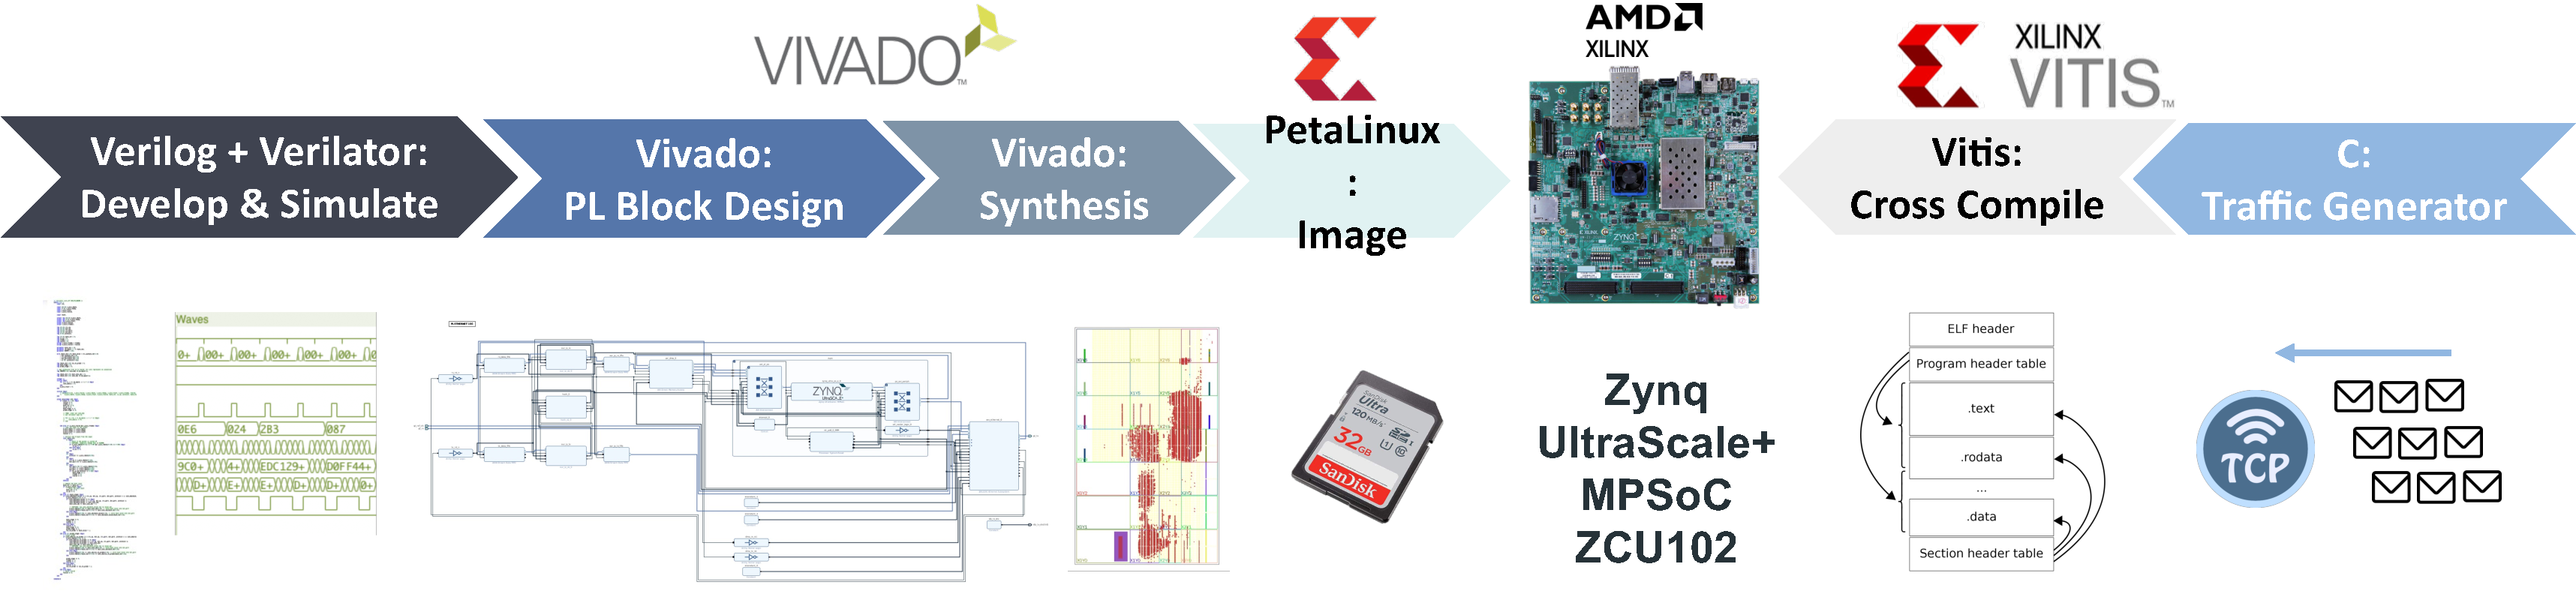
\includegraphics[width=500pt]{images/implworkflow.pdf}
    \caption{Our implementation workflow.}
    \label{fig:workflow}
    \Description{Implementation Workflow}
\end{figure*}

We elaborate on our detailed implementation workflow, including Verilog design and testing, Vivado block design, Petalinux image building, testbed deployment, and Vitis cross-compilation in this subsection. We used Vivado 19.02, Vitis 19.02, and Petalinux 19.02. Figure \ref{fig:workflow} illustrates our workflow.

\textbf{Hardware Implementation and Testing.} We utilized Verilog and Verilator to implement and test our design, consisting of approximately 300 lines of Verilog code and 1.5k lines of C++ code.

\begin{table}[h]
    \caption{ZCU102 Resource Consumption}
    \label{tab:res}
    \begin{tabular}{c|cccc}
      \toprule
        & LUT & FF & BRAM & DSP\\
      \midrule
      Original & 18923 & 18315 & 139.5 & 0\\
      Ours (table size 1024) & 33373 & 47067 & 142.0 & 0\\
      \midrule
      Ours / Total Resource (\%) & 12.18 & 8.59 & 15.57 & 0\\
      \bottomrule
  \end{tabular}
\end{table}

\begin{figure*}[t]
    \centering
    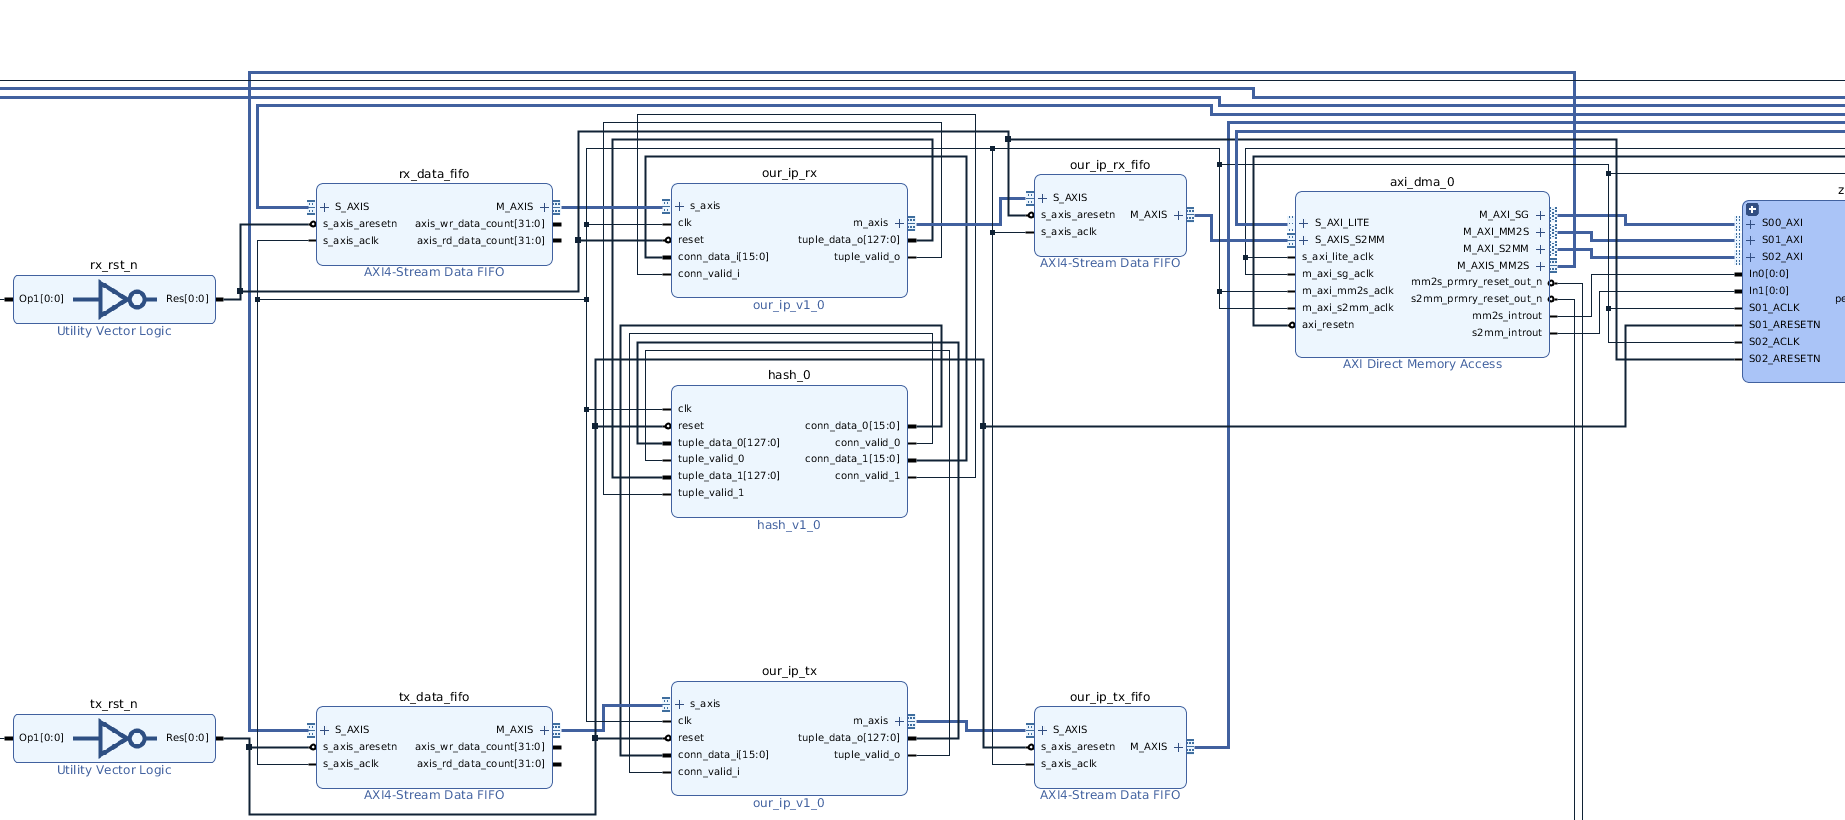
\includegraphics[width=400pt]{images/brd.png}
    \caption{The key part of our board design.}
    \label{fig:brd}
    \Description{Board Design}
\end{figure*}

\begin{figure}[t]
    \centering
    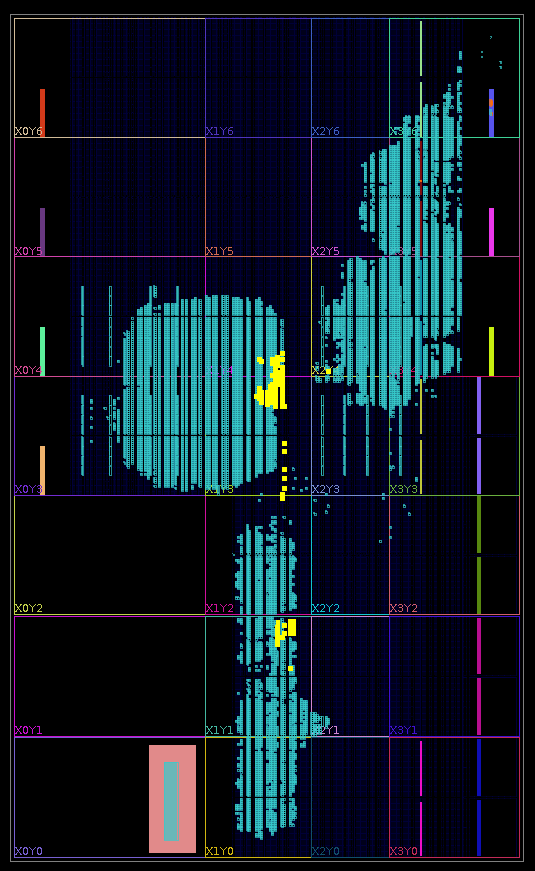
\includegraphics[width=\linewidth]{images/brdimpl.png}
    \caption{The post-synthesis netlist with the NAT part highlighted in yellow.}
    \label{fig:brdimpl}
    \Description{Post-synthesis Netlist}
\end{figure}

\textbf{Vivado Block Design and Synthesis.} We used Vivado to insert our Verilog implementation as custom IPs, and then synthesized, implemented, and generated a bitstream. Finally, we exported the hardware to an \verb|.xsa| file. The key part of our board design is shown in Figure \ref{fig:brd}, and the netlist is displayed in Figure \ref{fig:brdimpl}. Resource consumption details are presented in Table \ref{tab:res}. The entire design, including a table size of 1024 and the original 10/25G Ethernet Subsystem, consumes 12.18\% LUTs, 0.58\% LUTRAMs, 8.59\% FFs, and 15.57\% BRAMs.

\textbf{Petalinux Image Building.} Petalinux, a tool to build tiny embedded Linux images, was employed to build the images following the official tutorial in a Ubuntu 18.04 Docker container running on an AMD Ryzen 7 7700 (4.8 GHz full core). The image building process took several hours.

\textbf{Vitis Cross-Compilation.} To execute the C++ source code on the board's ARM cores, cross-compilation was necessary. Vitis provides cross-compilation support for various Zynq platforms, resulting in an ELF file that could be sent to the board via \verb|scp|.
